\documentclass[journal]{IEEEtran}
\usepackage[utf8]{inputenc}
\usepackage{graphicx}
\usepackage{amsmath}
\usepackage{siunitx}
\usepackage{xspace}
\usepackage{hyperref}
\usepackage{url}
\usepackage{cite}
\hyphenation{op-tical net-works semi-conduc-tor}

\begin{document}
	
	\title{Laboratorio 3: Lógica combinacional y Aritmética I}
	\author{Fiorella, Jonathan, Gerald}
	\date{Marzo 2021}
	
	\newcommand{\email}[1]{\href{mailto:#1}{#1}}
	
	\author{
		\IEEEauthorblockN
		{
			Fiorella Delgado León
			Jonathan Guzmán Araya,
			Gerald Valverde McKenzie
		}
		\IEEEauthorblockA{\\Instituto Tecnológico de Costa Rica}
		\IEEEauthorblockA{\\Área Académica Ingeniería en Computadores}
		
		\IEEEauthorblockA{\email{fiorelladelgado53@gmail.com}}		
		\IEEEauthorblockA{\email{jonathana1196@gmail.com}}
		\IEEEauthorblockA{\email{gvmckenzie@mckode.com}}
	}
	
	% The paper headers
	\markboth{Laboratorio Taller de Diseño Digital, Semestre I~2021}%
	{Shell \MakeLowercase{\textit{et al.}}: Bare Demo of IEEEtran.cls for IEEE Journals}
	
	
	% make the title area
	\maketitle
	
	% As a general rule, do not put math, special symbols or citations
	% in the abstract or keywords.
	\begin{abstract}

	\end{abstract}
	% Note that keywords are not normally used for peerreview papers.
	\begin{IEEEkeywords}
		ALU, compuertas lógicas, flip-flops, microprocesadores
	\end{IEEEkeywords}
	
	\section{Introducción}	
	Los circuitos combinacionales son aquellos en los que las salidas solo dependen solamente de las entradas, y no de ningún tipo de sincronización con señales de reloj, esto hace que los sistemas combinacionales sean generalmente rápidos. En sistemas digitales complejos, como los microprocesadores, los circuitos de lógica combinacional desempeñan un papel fundamental. La arquitectura de un microprocesador es como la que se observa en la Figura \ref{fig:microprocesador}.
	
	\begin{figure}[hbtp]
		\centering
		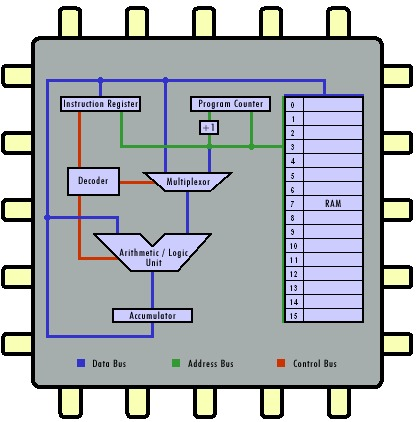
\includegraphics[scale = 0.5]{img/microprocesador.jpg}
		\caption{Arquitectura básica de un microprocesador \cite{Gonzalez2017}}
		\label{fig:microprocesador}
	\end{figure}
	
	Una función esencial de muchas computadoras (microprocesadores) y calculadoras es la realización de operaciones lógicas y aritméticas. Estas operaciones se efectúan en la unidad aritmética-lógica de una computadora, donde se combinan compuertas lógicas y flip-flops de manera que puedan sumar, restar, multiplicar y dividir números binarios \cite{Tocci2007}. El símbolo de una ALU es como el de la Figura \ref{fig:simboloalu}.
	
	\begin{figure}[!htb]
		\centering
		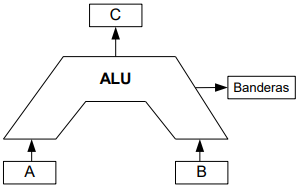
\includegraphics[scale = 0.5]{img/simboloalu.png}
		\caption{Símbolo ALU \cite{Garcia}}
		\label{fig:simboloalu}
	\end{figure}
	
	Además de los operadores lógicos, la ALU cuenta con una serie de registros para almacenar los datos y bits de información sobre los resultados, también llamados banderas \cite{Garcia}, las banderas más comunes en una ALU son: $Z$, $C$, $V$, $N$.
	\begin{itemize}
		\item Zero flag: usada para determinar si dos valores son iguales, generalmente se usa una resta, y se revisa si el resultado es cero, si es así, esta bandera se enciende.
		\item Overflow flag: usada para determinar si el resultado de una operación (usualmente suma o multiplicación), tiene un tamaño superior al máximo representable, o inferior al mínimo representable en la ALU, es posible que existan como banderas separadas.
		\item Negative flag: usada para determinar si el resultado de una resta es menor a cero
		\item Carry/Borrow flag: Esta bandera indica cuando una operación  resulta en un valor más largo del cual el acumulador puede representar o menor del cual el acumulador puede representar.
	\end{itemize}
	
	La ALU es simplemente un operador, es decir solo realiza operaciones, esta no toma decisiones, acepta datos binarios que están almacenados en la memoria y ejecuta operaciones con estos datos, de acuerdo a las instrucciones que vienen de la unidad de control.
	
	Para realizar operaciones lógicas la ALU utiliza compuertas lógicas como:
	
	\begin{itemize}
		\item NOT: La Figura \ref{fig:NOT} muestra el símbolo para un circuito NOT, la operación NOT cambia de un nivel lógico al nivel lógico opuesto. Cuando la entrada está a nivel ALTO (1), la salida se pone a nivel BAJO (0). Cuando la entrada está a nivel BAJO, la salida se pone a nivel ALTO \cite{Floyd2006}.
		
		\begin{figure}
			\centering
			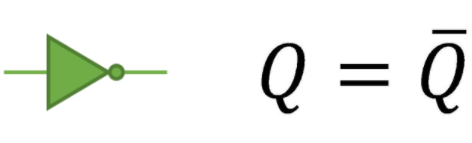
\includegraphics[scale = 0.5]{img/NOT.png}
			\caption{Compuerta NOT y su representación en álgebra de Boole \cite{Tocci2007}}
			\label{fig:NOT}
		\end{figure}
		
		\begin{table}[!htb]
			\centering
			\begin{tabular}{|c|c|}
				\hline
				Q & Q' \\
				\hline
				\hline
				0 & 1 \\
				\hline
				1 & 0 \\
				\hline
			\end{tabular}
			\caption{Tabla de verdad de la compuerta NOT}
			\label{tab:NOT}
		\end{table}
		
		\item AND: La Figura \ref{fig:AND} muestra el símbolo lógico para una compuerta AND de dos entradas. La operación AND genera un nivel ALTO sólo cuando todas las entradas están a nivel ALTO, para el caso de dos entradas. Cuando una entrada está a nivel ALTO y la otra entrada está a nivel ALTO, la salida se pone a nivel ALTO. Cuando cualquiera de las entradas o todas ellas están a nivel BAJO, la salida se pone a nivel BAJO \cite{Floyd2006}.
		
		\begin{figure}[!htb]
			\centering
			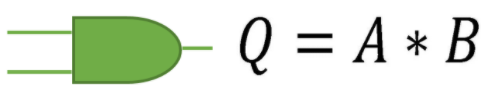
\includegraphics[scale = 0.3]{img/AND.png}
			\caption{Compuerta AND y su representación en álgebra de Boole \cite{Tocci2007}}
			\label{fig:AND}
		\end{figure}
		
		\begin{table}[!htb]
			\centering
			\begin{tabular}{|c|c|c|}
				\hline
				A & B & Q \\
				\hline
				\hline
				0 & 0 & 0 \\
				\hline
				0 & 1 & 0 \\
				\hline
				1 & 0 & 0 \\
				\hline
				1 & 1 & 1 \\
				\hline
			\end{tabular}
			\caption{Tabla de verdad de la compuerta AND}
			\label{tab:AND}
		\end{table}
		
		\item OR: La Figura \ref{fig:OR} muestra el símbolo lógico para una compuerta OR de dos entradas. La operación OR genera un nivel ALTO cuando una o más entradas están a nivel ALTO, para el caso de dos entradas. Cuando una de las entradas está a nivel ALTO o ambas entradas
		están a nivel ALTO, la salida es un nivel ALTO. Cuando ambas entradas están a nivel BAJO, la salida será un nivel BAJO \cite{Floyd2006}.
		
		\begin{figure}[!htb]
			\centering
			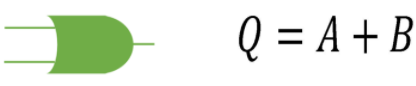
\includegraphics[scale = 0.35]{img/OR.png}
			\caption{Compuerta OR y su representación en álgebra de Boole \cite{Tocci2007}}
			\label{fig:OR}
		\end{figure}
		
		\begin{table}[!htb]
			\centering
			\begin{tabular}{|c|c|c|}
				\hline
				A & B & Q \\
				\hline
				\hline
				0 & 0 & 0 \\
				\hline
				0 & 1 & 1 \\
				\hline
				1 & 0 & 1 \\
				\hline
				1 & 1 & 1 \\
				\hline
			\end{tabular}
			\caption{Tabla de verdad de la compuerta OR}
			\label{tab:OR}
		\end{table}
		
		\item XOR: La Figura \ref{fig:XOR} muestra el símbolo lógico para una compuerta XOR de dos entradas. En una compuerta OR-exclusiva, la salida X es un nivel ALTO si la entrada A está a nivel BAJO y la entrada B está a nivel ALTO; o si la entrada A está a nivel ALTO y la entrada B está a nivel BAJO; X es un nivel BAJO si tanto A como B están a nivel ALTO o BAJO \cite{Floyd2006}.
		
		\begin{figure}[!htb]
			\centering
			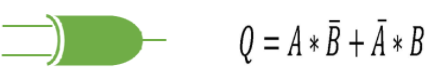
\includegraphics[scale = 0.4]{img/XOR.png}
			\caption{Compuerta XOR y su representación en álgebra de Boole \cite{Tocci2007}}
			\label{fig:XOR}
		\end{figure}
		
		\begin{table}[!htb]
			\centering
			\begin{tabular}{|c|c|c|}
				\hline
				A & B & Q \\
				\hline
				\hline
				0 & 0 & 0 \\
				\hline
				0 & 1 & 1 \\
				\hline
				1 & 0 & 1 \\
				\hline
				1 & 1 & 0 \\
				\hline
			\end{tabular}
			\caption{Tabla de verdad de la compuerta XOR}
			\label{tab:XOR}
		\end{table}
	\end{itemize}
	
	
	
	Uno de los problemas más desafiantes en el diseño de circuitos es el tiempo, hacer que un circuito funcione rápido. Una salida necesita tiempo para cambiar en respuesta a un cambio en la entrada, como se observa en la Figura \ref{fit:delay} \cite{SarahL.Harris2010}.
	
	\begin{figure}[hbtp]
		\centering
		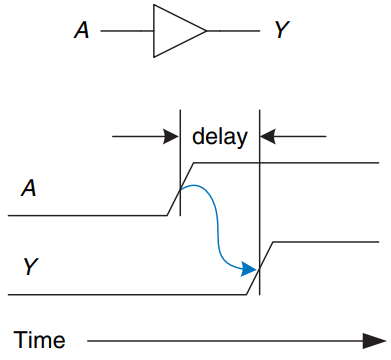
\includegraphics[scale = 0.4]{img/delay.png}
		\caption{Tiempo de respuesta de una señal \cite{SarahL.Harris2010}}
		\label{fit:delay}
	\end{figure}

	En la lógica combinacional existen dos tipos de tiempos, tiempo de propagación y tiempo de contaminación. El tiempo de propagación $t_{pd}$ es el tiempo máximo desde que la entrada cambia hasta que el o las salidas llegan a su valor final y el tiempo de contaminación $t_{cd}$ es el tiempo mínimo que dura la entrada en cambiar hasta que alguna salida empiece a cambiar su valor \cite{SarahL.Harris2010}.
	
	Además de los tiempos de propagación y contaminación en la electrónica de circuitos existe algo llamado la ruta crítica, que es la ruta más larga que tiene una entrada, hablando de circuitos combinacionales, para llegar a la salida, por lo tanto, esta ruta también sería la más lenta. Ahora para describir a un circuito hay dos factores muy importantes: latencia y tasa de transferencia. La latencia funcionaria como la frecuencia del circuito, ya que es el tiempo que se necesita para que el cambio en la entrada haga un cambio en la salida; esta puede ser expresada en tiempo o, para circuitos sincrónicos, un cierto número de ciclos de reloj.  Y la tasa de transferencia a la velocidad con la que la información puede ser procesada. Por ejemplo, en la Figura \ref{fig:criticalpath} se tienen tres rutas distintas desde una entrada hasta la salida, siendo la ruta azul la más lenta de estas.
	
	\begin{figure}[hbtp]
		\centering
		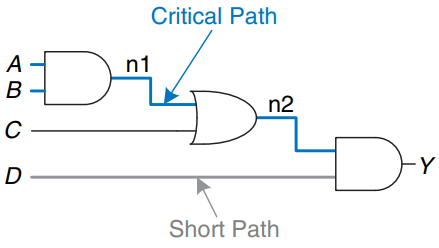
\includegraphics[scale = 0.4]{img/criticalpath.png}
		\caption{Ruta crítica \cite{SarahL.Harris2010}}
		\label{fig:criticalpath}
	\end{figure}

	Así el tiempo de propagación de un circuito combinacional es la suma de los tiempos de propagación de cada elemento que lo compone como se observa en la Ecuación \ref{eq:tpd} y el tiempo de contaminación es la suma de los tiempos de contaminación de la más corta del circuito combinacional que se puede observar en la Ecuación \ref{eq:tcd}.
	
	\begin{equation}
		t_{pd} = 2t_{pdAND} + t_{pdOR}
		%\caption{Tiempo de propagación del circuito}
		\label{eq:tpd}
	\end{equation}

	\begin{equation}
		t_{pd} = 2t_{pdAND} + t_{pdOR}
		%\caption{Tiempo de contaminación del circuito}
		\label{eq:tcd}
	\end{equation}

	En circuitos más complejos como un procesador pipeline como el de la Figura \ref{fig:pipe}, la velocidad de ciclos del reloj decrece haciendo retrasos en la ruta crítica, para esto se utiliza la técnica de Pipelining, el cual consiste en dividir el circuito en varias partes con un registro al final de cada una, de esta manera se divide la ruta crítica en pequeñas rutas, permitiendo que la velocidad del reloj aumente y consecuentemente también lo haga la tasa de transferencia. La segmentación consiste en descomponer la ejecución de cada instrucción en varias etapas para poder empezar a procesar una instrucción diferente en cada una de ellas y trabajar con varias a la vez. Las etapas de segmentación pueden ser: IF (búsqueda), ID (decodificación), EX (ejecución), MEM (memoria), WB (escritura), en una arquitectura relativamente sencilla.
	
	\begin{figure}[hbtp]
		\centering
		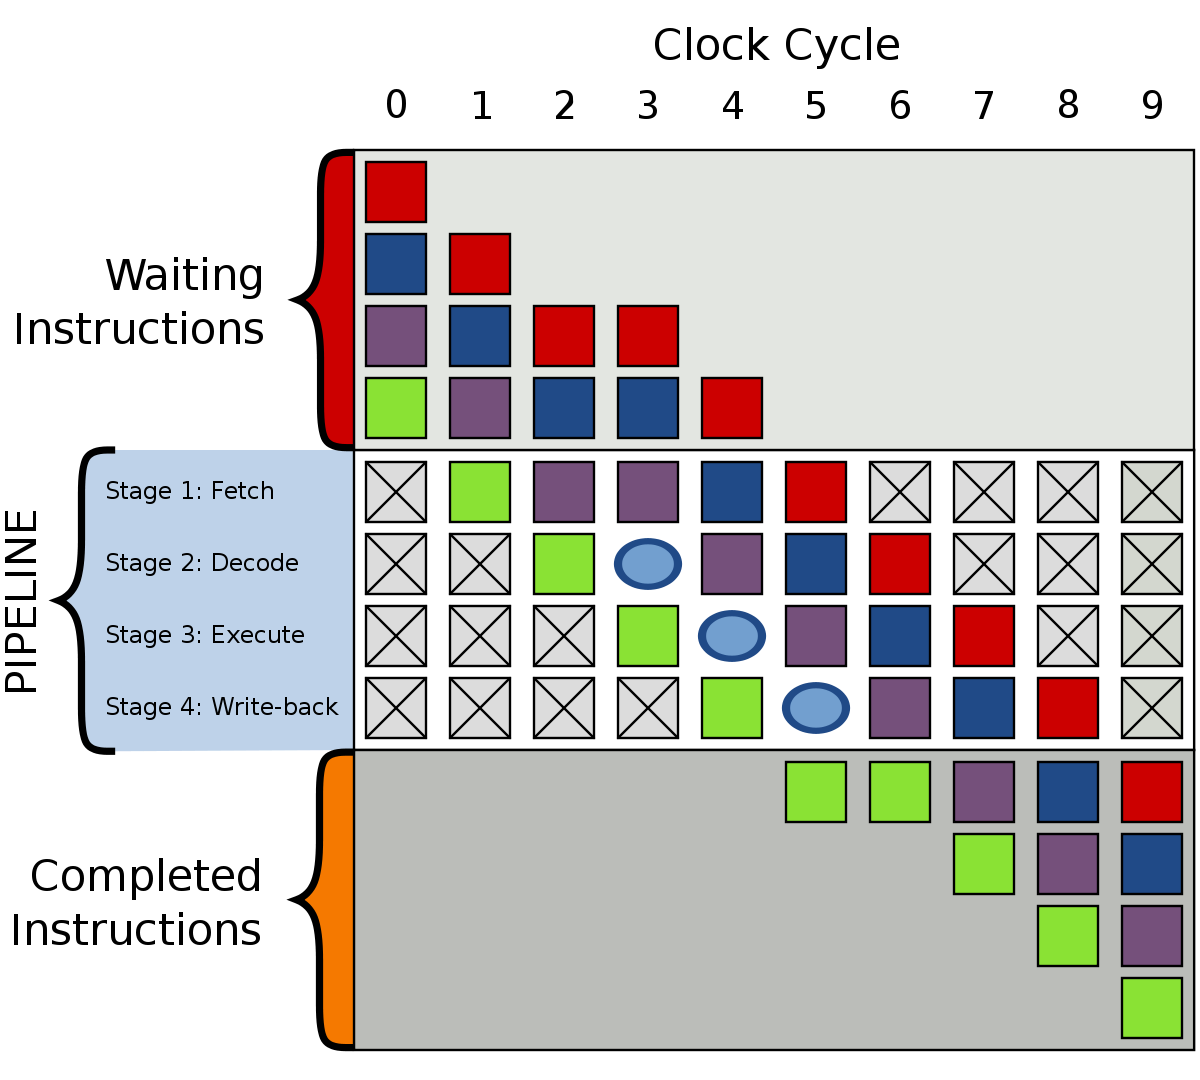
\includegraphics[scale = 0.15]{img/Pipe.jpg}
		\caption{Procesador Pipeline \cite{pipewiki}}
		\label{fig:pipe}
	\end{figure}

	La frecuencia máxima de operación de un circuito está determinada por la ruta crítica del mismo, para esto se toma la ruta crítica (en un procesador se realiza tomando la instrucción que tarda más en ejecutarse por completo sin afectar a las otras) y se calcula el tiempo que tarda en ciclos de reloj $T_{c}$, como se observa en la Ecuación \ref{eq:fHz}, esta frecuencia se mide en $Hz$.
	
	\begin{equation}
		f_{c} = \dfrac{1}{T_{c}}
		%\caption{Frecuencia de un circuito}
		\label{eq:fHz}
	\end{equation}


	\section{Desarrollo}

	Para el desarrollo de este laboratorio, se realizó la implementación de dos soluciones a dos problemas por medio del lenguaje System Verilog.

	\subsection{Experimento 1}
	
	El primer experimento del laboratorio consiste en la implementación de una Unidad Lógica Aritmética. Dicha unidad debe realizar una serie de operaciones, siendo una calculadora parametrizable de manera que la cantidad de bits de entrada puedan ser modificados.
	En la Figura MOOOOOODIFICAR se observan las diversas operaciones y los valores de la entrada de selección para ejecutar dicha operación. Así mismo la ALU es implementada con banderas de estado tales como: Negativo (N), Cero (Z), Acarreo (C) y Desbordamiento (V).
	
	\begin{table}[hbtp]
		\begin{center}
			\caption{Tabla de las operaciones con su respectivo selector.}
			\label{tab:tabla1}
			
			\begin{tabular}{c | c }
				\hline
				\textbf{Operación} & \textbf{Selector} \\
				\hline Suma & 0000   \\
				\hline  Resta & 0001   \\
				\hline Multiplicación & 0010   \\
				\hline División Q1 & 0011   \\
				\hline Módulo Q3 & 0100   \\
				\hline AND & 0101   \\
				\hline OR & 0110   \\
				\hline XOR & 0111   \\
				\hline Shift Left & 1000   \\
				\hline Shift Right & 1001   \\
			\end{tabular}
		\end{center}
	\end{table}

	La ALU fue implementada mediante el modelado estructural, en donde se utilizan módulos independientes para llegar a formar la ALU completamente.
	
	
	
	En la Figura \ref{fig:niv11}, se puede observar el diagrama de primer nivel de la calculadora parametrizable, en donde las entradas A y B, son los dos datos de entrada que van a ser operados, para este caso pueden ser de N bits; la entrada S, es la entrada de selección, la cual se utiliza para escoger la operación que se desea aplicar a los dos operandos ingresados (A y B), para este caso y con las operaciones que puede realizar esta calculadora.
	
	
	\begin{figure}[hbtp]
		\centering
		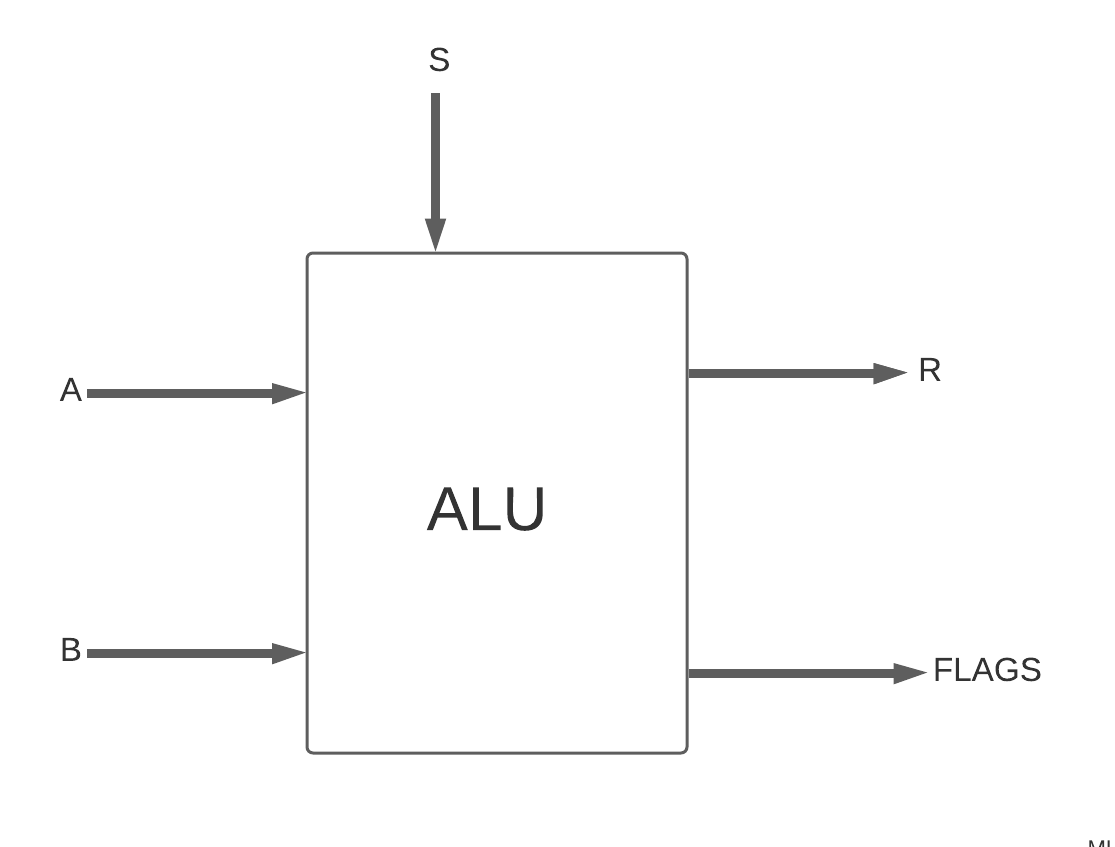
\includegraphics[scale = 0.4]{img/Nivel11.png}
		\caption{Diagrama de primer nivel de la calculadora parametrizable }
		\label{fig:niv11}
	\end{figure}
	
	La salida Q es el resultado generado por la ALU al operar los datos ingresados, dicha salida es de 4 bits. Por otro lado, la salida FLAGS es un bit array que posee cada una de las banderas de estado implementadas por lo tanto es una salida de 4 bits. 
	\subsubsection{Restricciones de diseño}
	\begin{itemize}
		\item La ALU implementada posee una salida Q de 4 bits por lo cuál cualquier dato mayor a este que se desee visualizar a la salida de la calculadora, se verá demostrado por la flag V.
		\item Tanto el sumador como el restador son implementados por medio de un modelo estructural, por lo cuál sus entradas no son parametrizables, siendo estas de 4 bits cada una.
		\item La operación de resta sólo admite números positivos en sus operandos siendo el resultado $Q=A-B$.
	\end{itemize}
	\subsubsection{Implementación}
	
	La estructura interna de la ALU consiste en una estructura modular en la que se compone de diversos módulos. En la Figura \ref{fig:d2}, se logra apreciar como los diferentes subsistemas interactúan entre sí. Por otro lado, en la Figura \ref{fig:d3}, se observa el diagrama de tercer nivel del dispositivo siendo este con mayor detalle, en donde hay 10 módulos que representan cada una de las operaciones, recibiendo de entrada A y B, dando como resultado una señal $I_i$. Las señales $I_i$, son los datos de entrada para el MUX encargado de filtrar el dato que se va mostrar a la salida por medio de los bits de entrada de la señal S.
	\begin{figure}[hbtp]
		\centering
		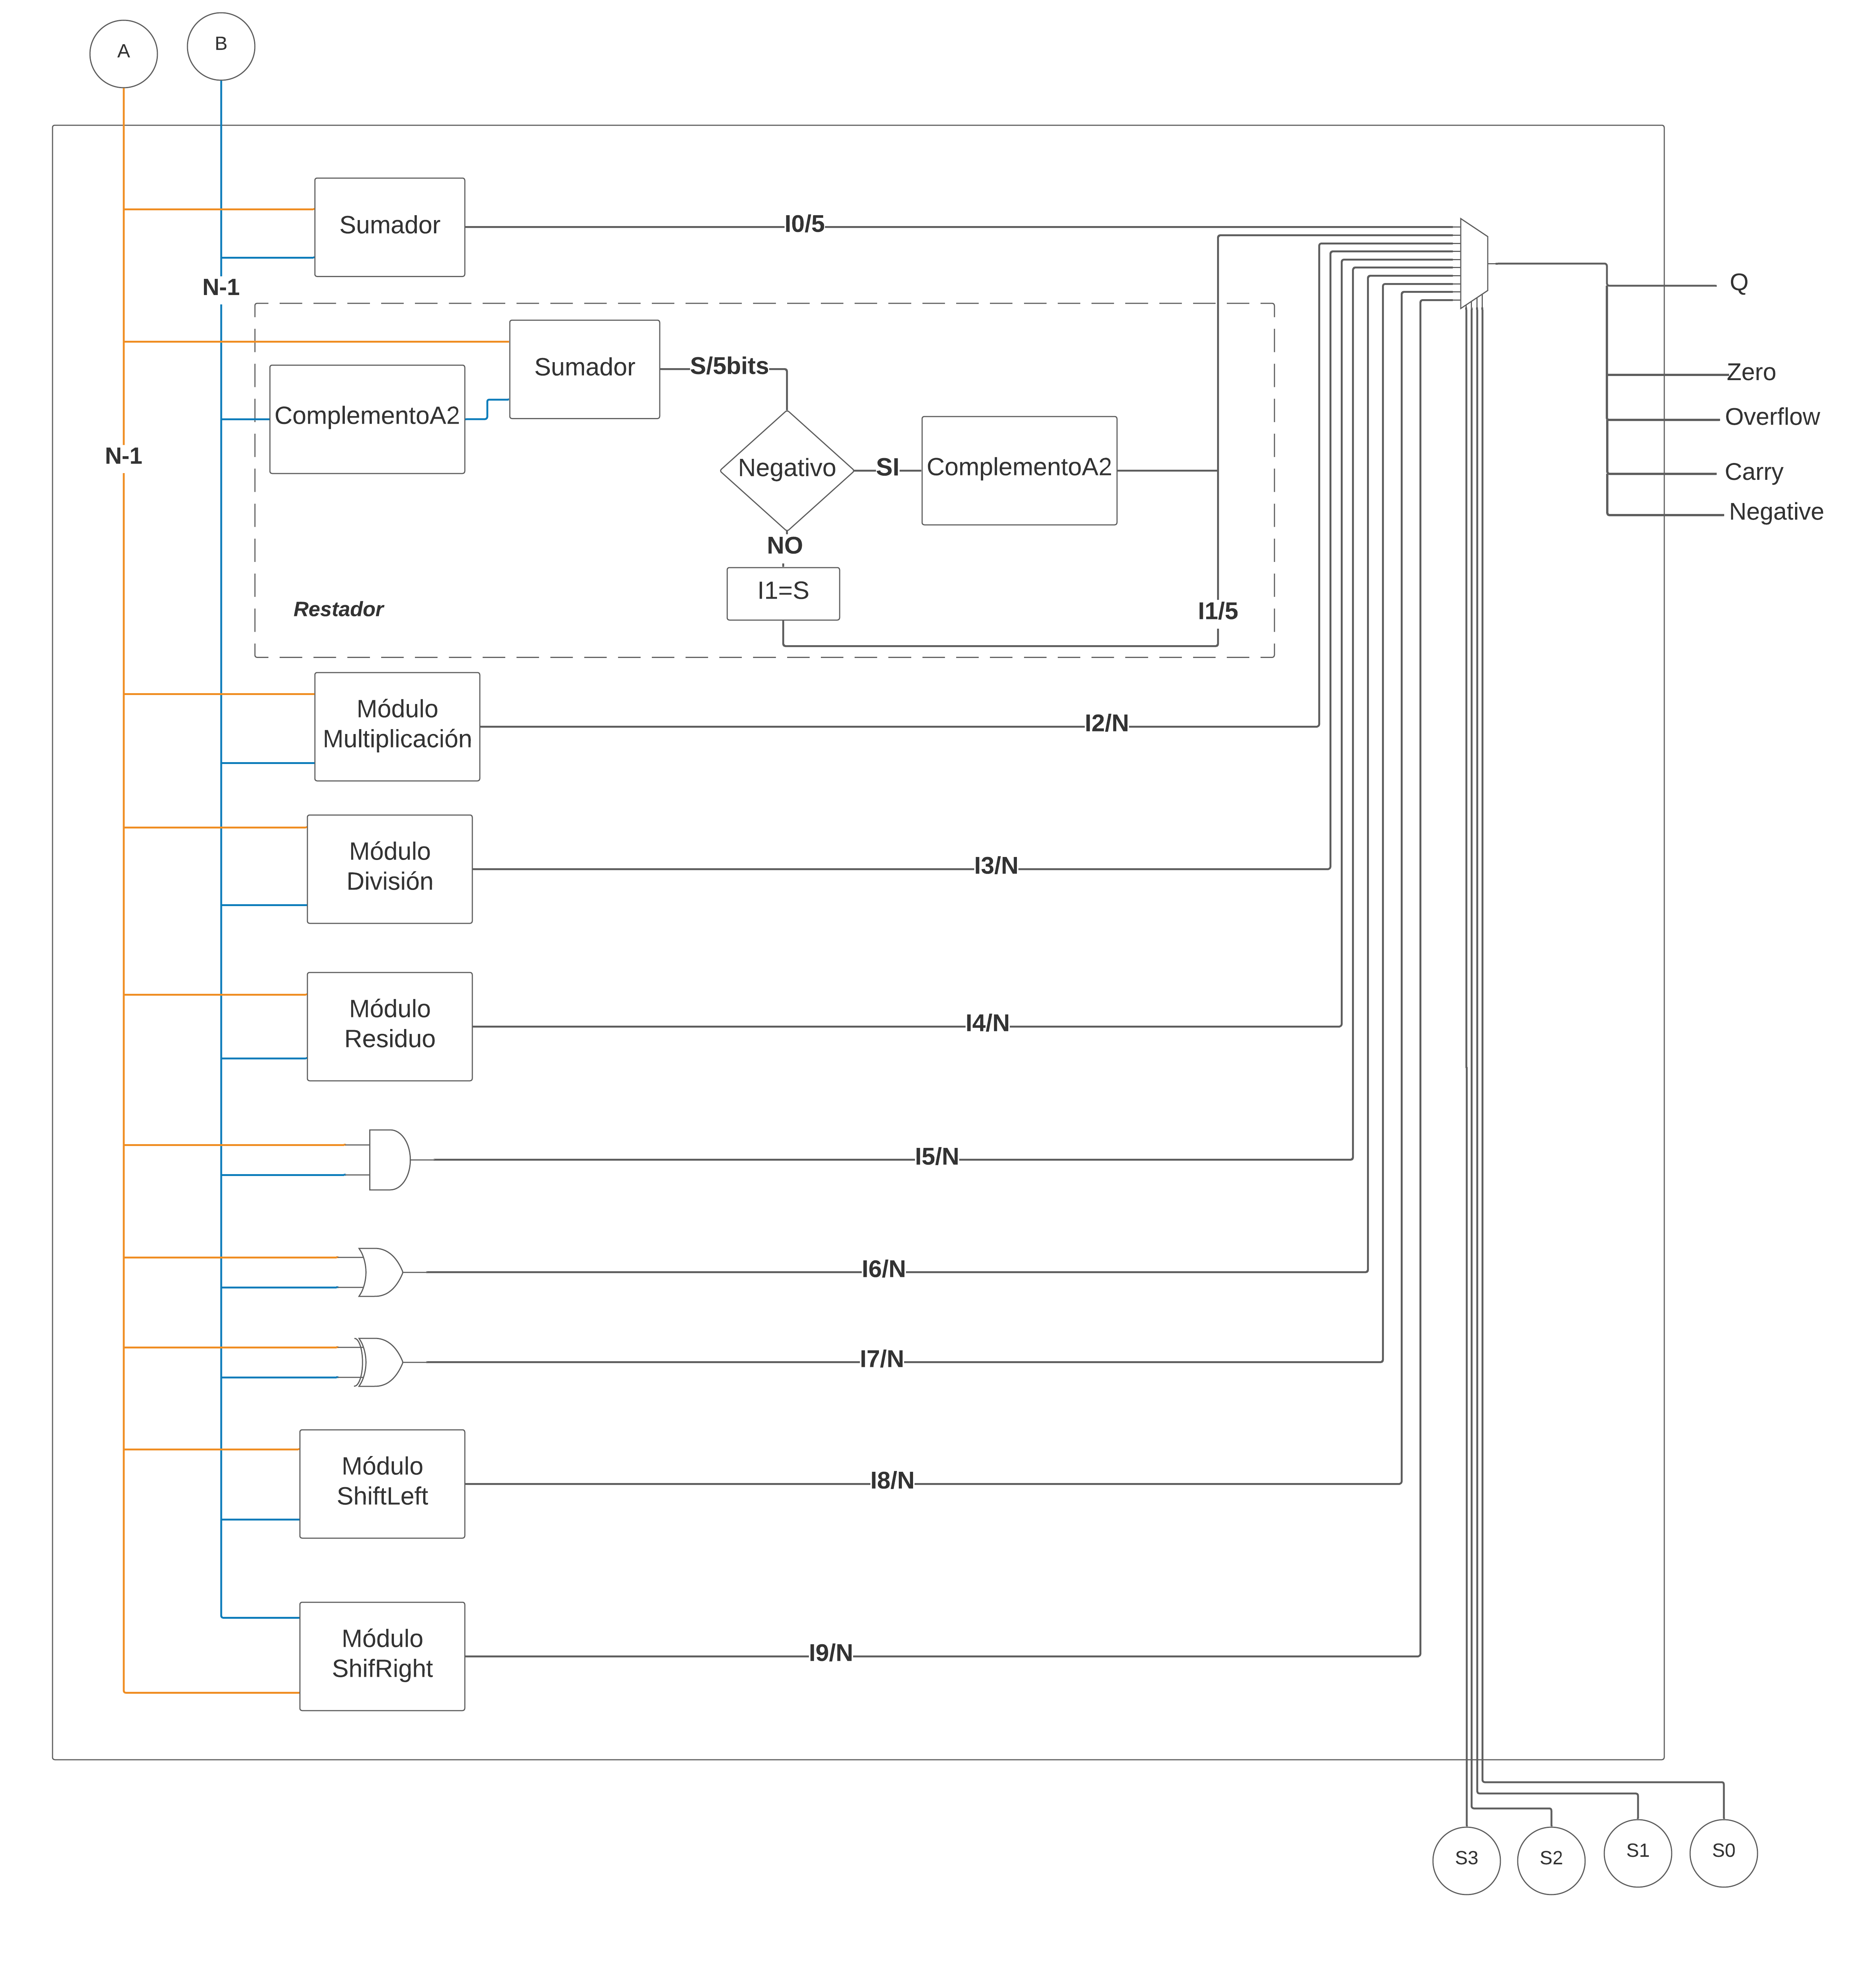
\includegraphics[scale = 0.04]{img/segundonivel.png}
		\caption{Diagrama de segundo nivel de la ALU }
		\label{fig:d2}
	\end{figure}
	
	\begin{figure}[hbtp]
		\centering
		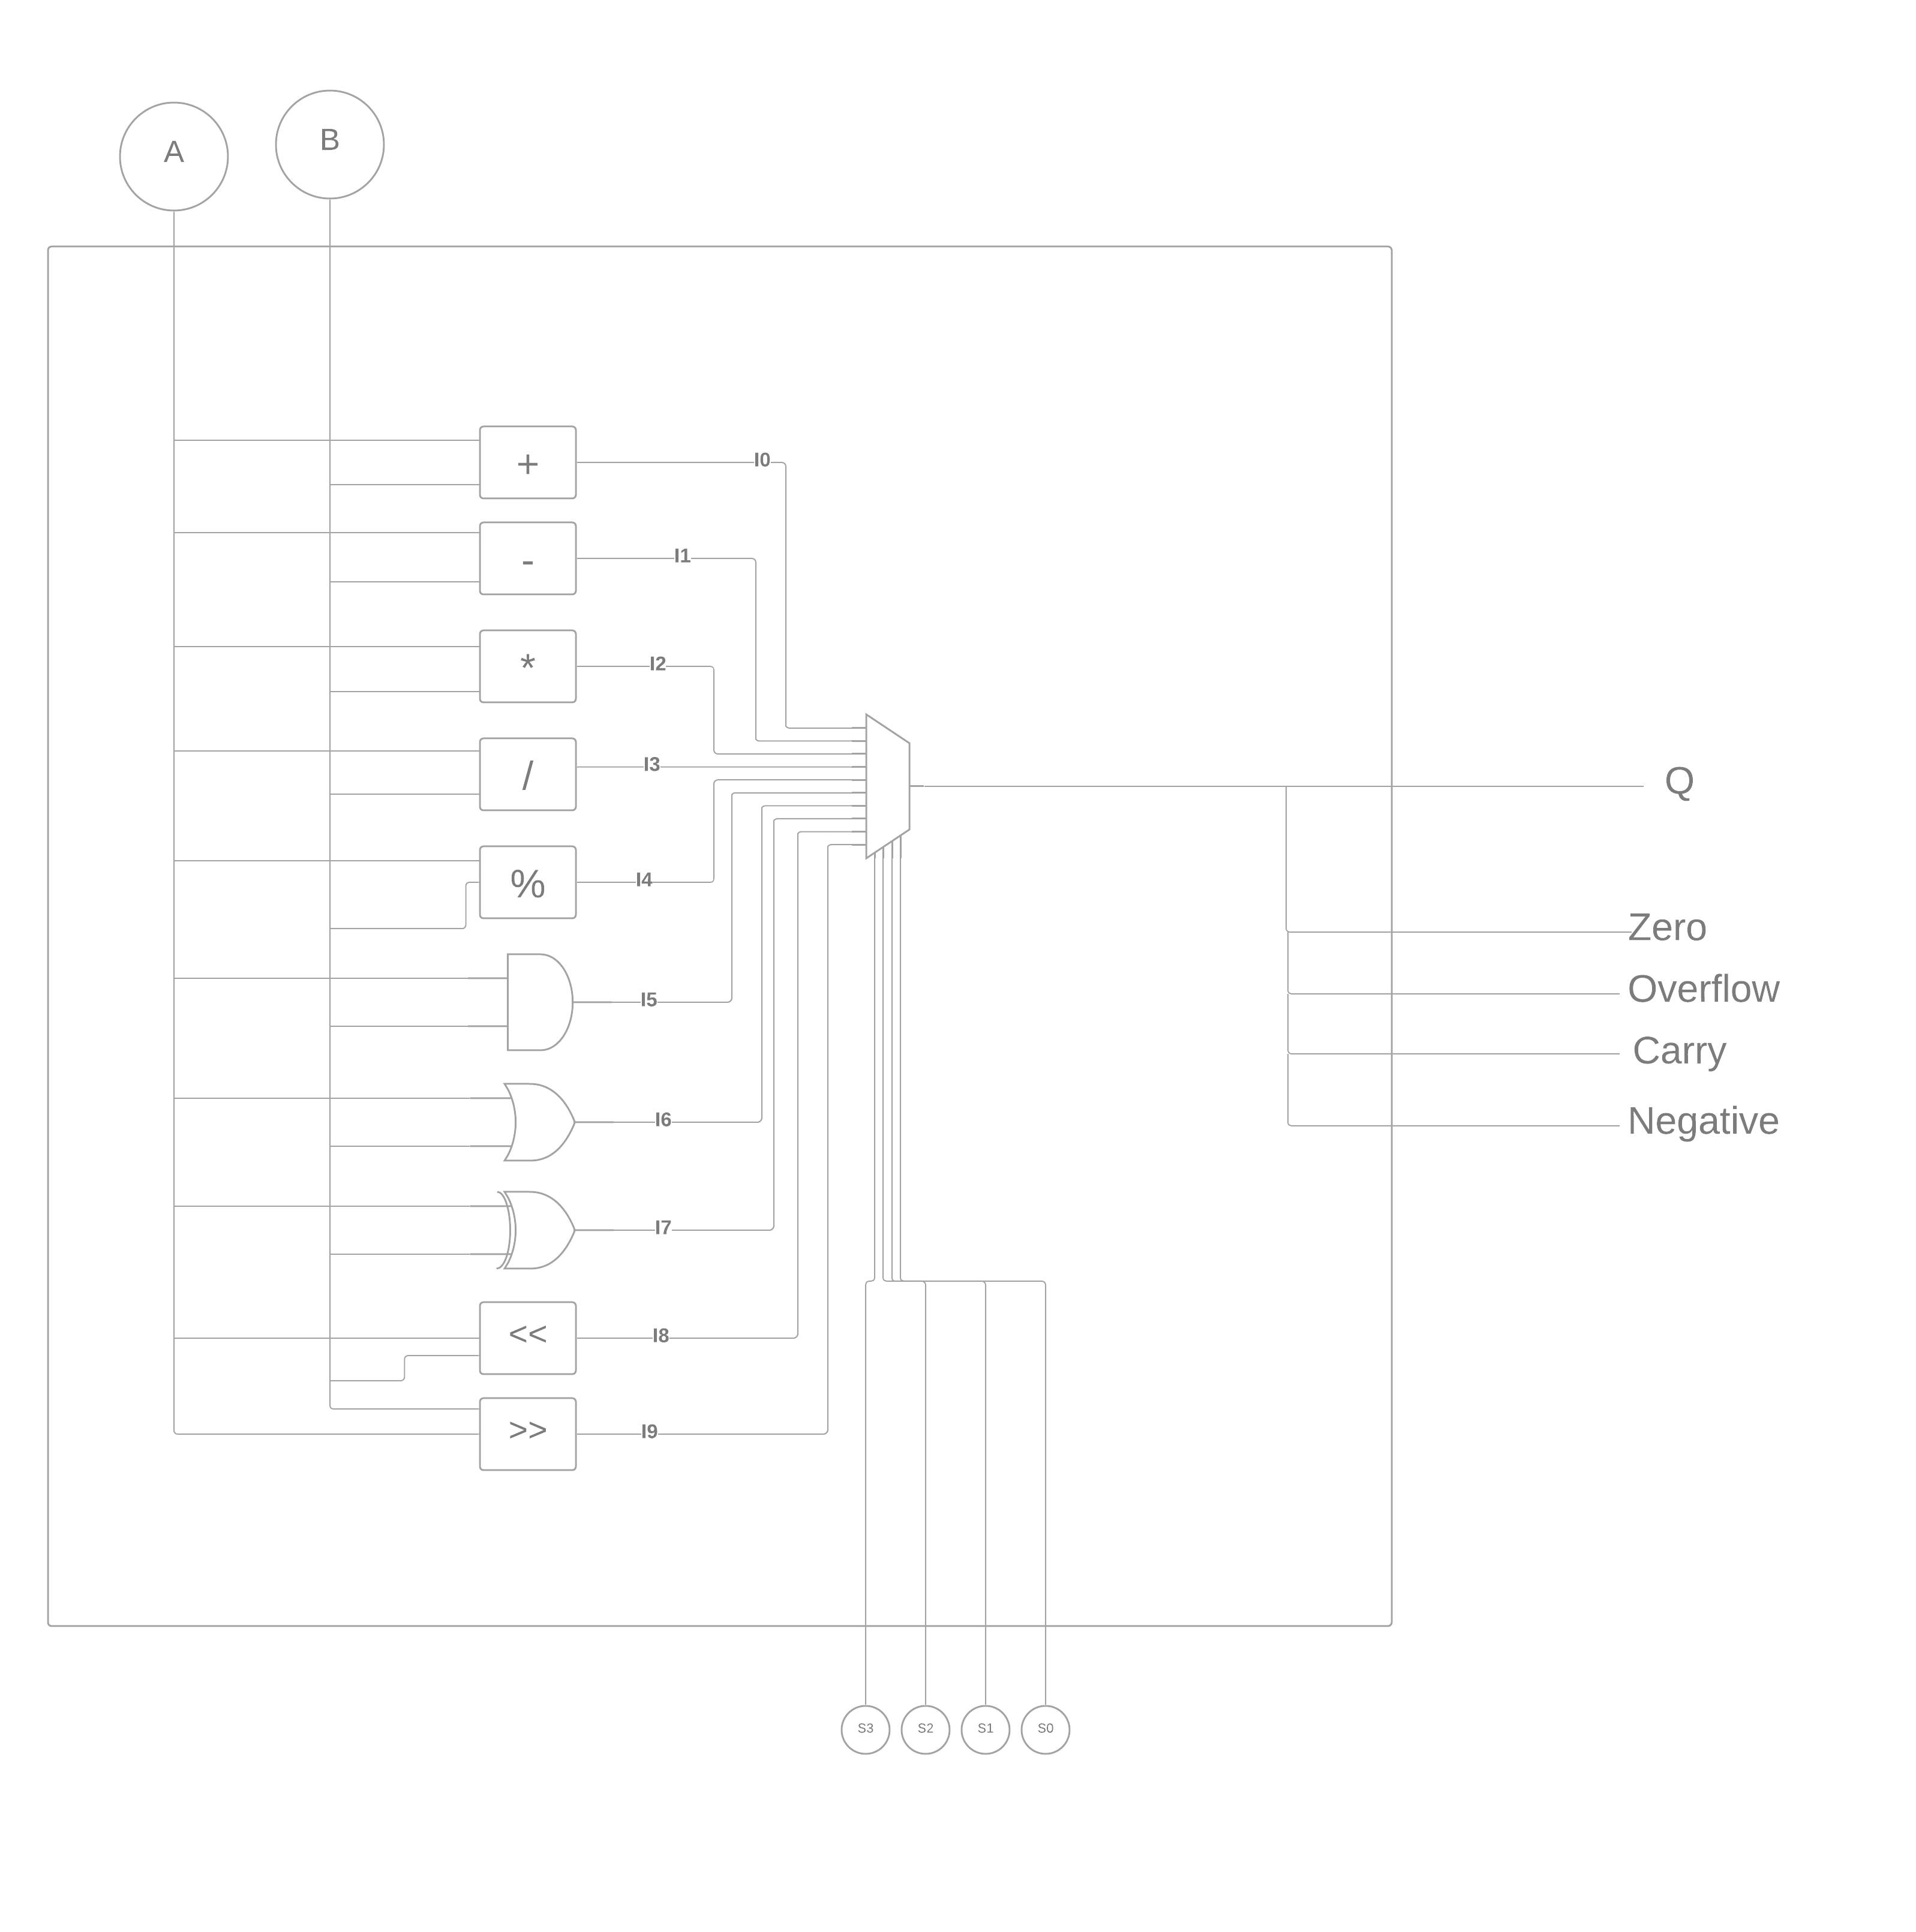
\includegraphics[scale = 0.07]{img/tercernivel.png}
		\caption{Diagrama de tercer nivel de la implementación de la ALU }
		\label{fig:d3}
	\end{figure}
	
	Tal como se menciona en las restricciones del experimento 1, tanto el sumador como el restador han sido implementados por medio del modelo estructural. Por lo que el sumador de 4 bits ha sido desarrollado conectando 4 sumadores completos de 1 bit (véase la estructura interna de este en la Figura \ref{fig:sum1}) en forma de cascada tal como se observa en la Figura \ref{fig:sum4}, en donde los datos $A_i$ representan cada uno de los bits de entrada del primer operando siendo $A_0$ el LSB, así mismo las señales $B_i$ representan los datos de la segunda entrada. Las señales $S_i$ representa el resultado del sumador y $C_o$ es el acarreo de salida o Carry Output. Para fines de diseño se definió como quinto bit de la señal S. 
	
	\begin{figure}[hbtp]
		\centering
		\includegraphics[scale = 0.13]{img/Sumador1.png}
		\caption{Diagrama lógico de un sumador de 1 bit }
		\label{fig:sum1}
	\end{figure}
	
	
	\begin{figure}[hbtp]
		\centering
		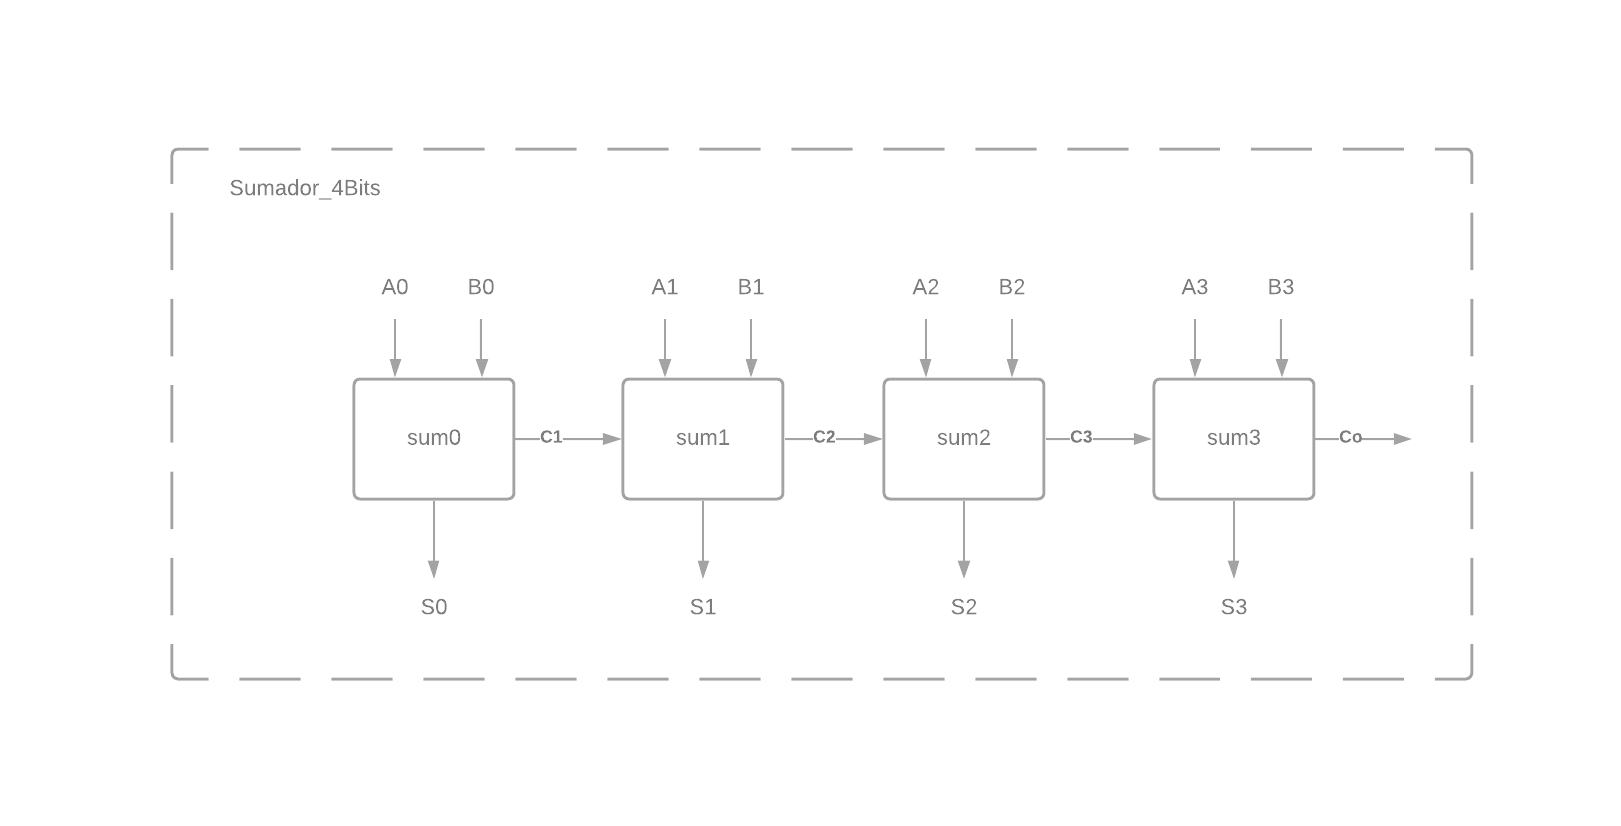
\includegraphics[scale = 0.15]{img/sumador4.png}
		\caption{Diagrama del modelo estructural de un sumador de 5 bits }
		\label{fig:sum4}
	\end{figure}
	
	
	En cuanto a la implementación del restador se le aplica el complemento A2 al segundo operando B, seguidamente se realiza la operación de $A+ComplementoA2(B)$, se procede analizando signo del resultado siendo este el MSB, si el signo de la operación es negativo se procede a realizar el complemento A2 al resultado, en el caso que el signo sea positivo se mantiene sin cambios, tal como se muestra en la Figura \ref{fig:rest4}.
	
	\begin{figure}[hbtp]
		\centering
		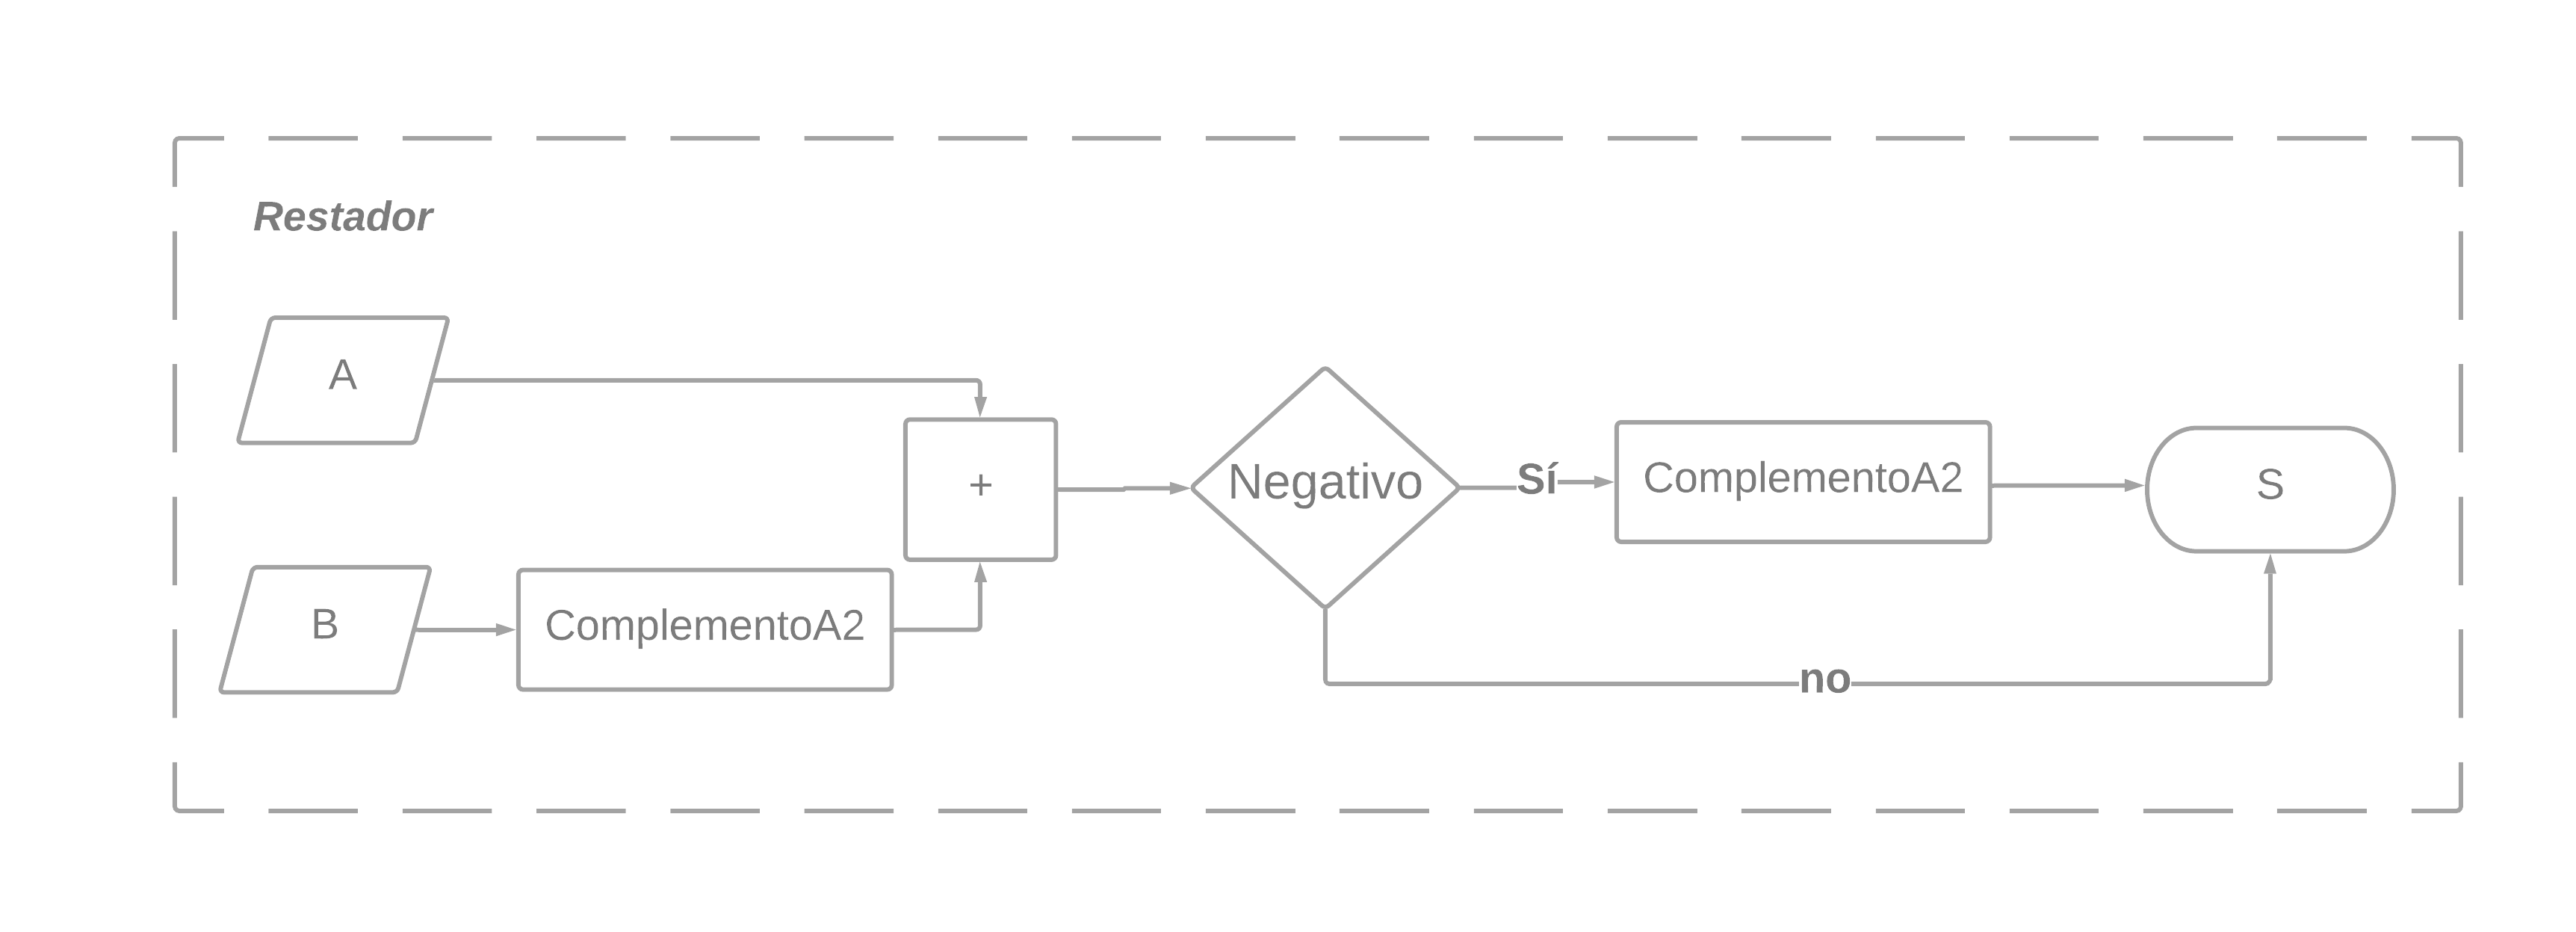
\includegraphics[scale = 0.07
		]{img/rest.png}
		\caption{Diagrama de flujo del restador de 4 bits }
		\label{fig:rest4}
	\end{figure}
	
	
	Finalmente, para la implementación en la FPGA se implementa el diagrama resultante de la Figura \ref{fig:alufpga}, el cuál consiste en la representación de los datos por medio de un displays. Siendo la salida de 4 bits el caso extremo a representar corresponde a la salida $Q=1111$ siendo su representación en decimal de $Q=15$, siendo este un número de dos dígitos (decenas y unidades) por lo que se decide la implementación de un display para cada dígito. Para realizarlo, se procede a calcular las unidades con la operación $Q\%10$, así mismo se procede con el cálculo de las decenas por medio de $Q//10$. Las salidas de dichas operaciones son enviadas a un decodificador el cuál se encarga de convertir el número binario que representa cada dígito decimal a un arreglo de 7 bits que corresponde a la elaboración de la representación en el display de 7 segmentos.
	
	\begin{figure}[hbtp]
		\centering
		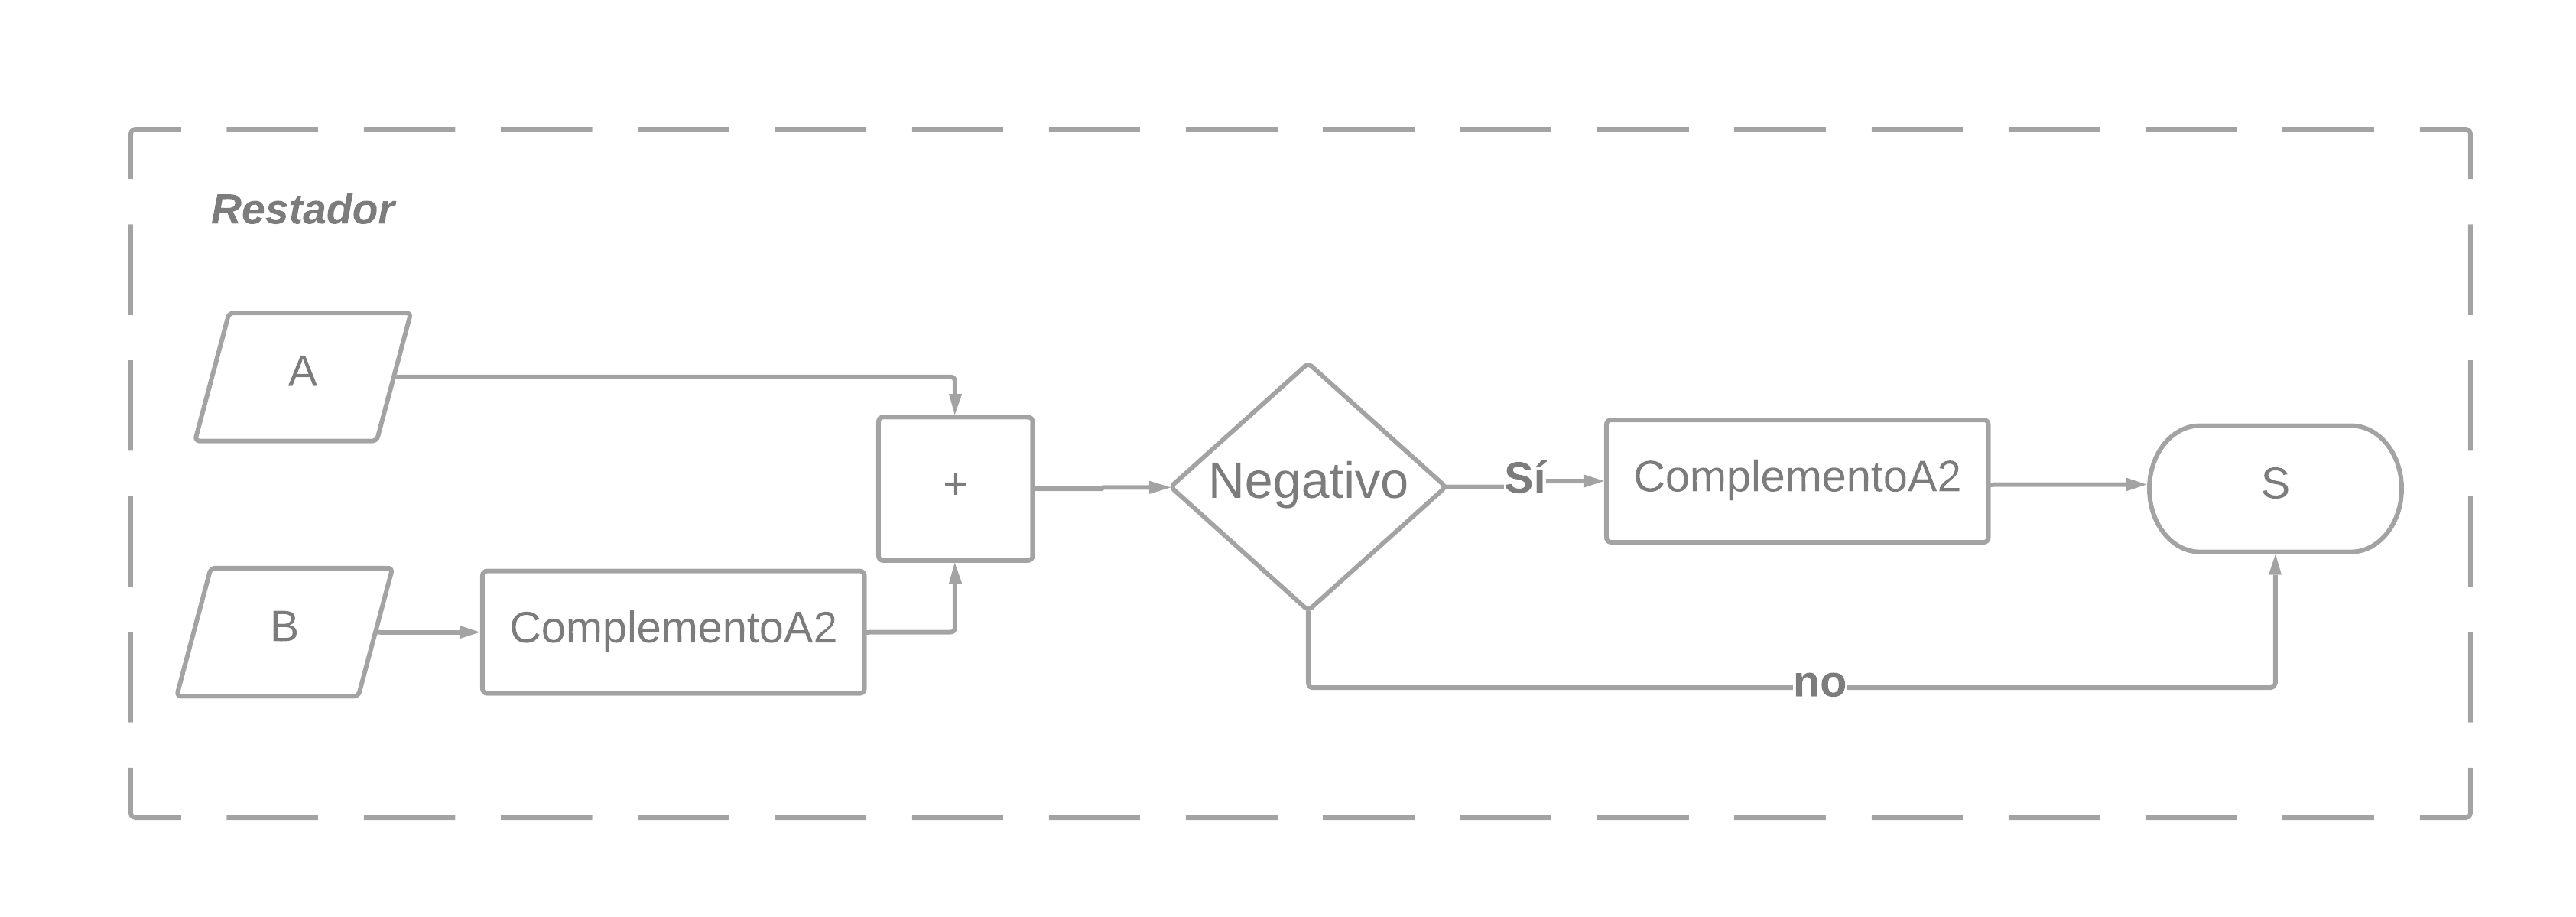
\includegraphics[scale = 0.07]{img/alu_fpga.png}
		\caption{Diagrama de la implementación de la ALU en la FPGA}
		\label{fig:alufpga}
	\end{figure}
	
	
	\subsection{Experimento 2}
	En este experimento, se requiere implementar dos registros de carga paralela entre la ALU; esto con el fin de determinar la frecuencia máxima a la que puede operar un reloj. En esta implementación se desarrollaron 5 test-bench en donde se comprueba el funcionamiento del ALU con 5, 32, 64, 128 y 256 bits.
	
	En la Figura \ref{fig:niv12}, se puede observar cómo el circuito electrónico parametrizable para la medición de frecuencia máxima de operación tiene 4 entradas que son ingresadas externamente mediante el uso de switches y botones; la entrada E0 (Dato de entrada) es de n bits, la entrada E1 (Reset1) es el reset para el primer registro es de 1 bit, la entrada E2 (Reset2) es el reset para el segundo registro es de 1 bit y la entrada E3 (Clock) es una entrada en común de reloj para ambos registros y es de 1 bit. Por otro lado, el mismo circuito sólo posee una salida la cual es el Resultado (S0) y es de n bits, este hace referencia al resultado de operar los dos números en el ALU.
	
	
	\begin{figure}[hbtp]
		\centering
		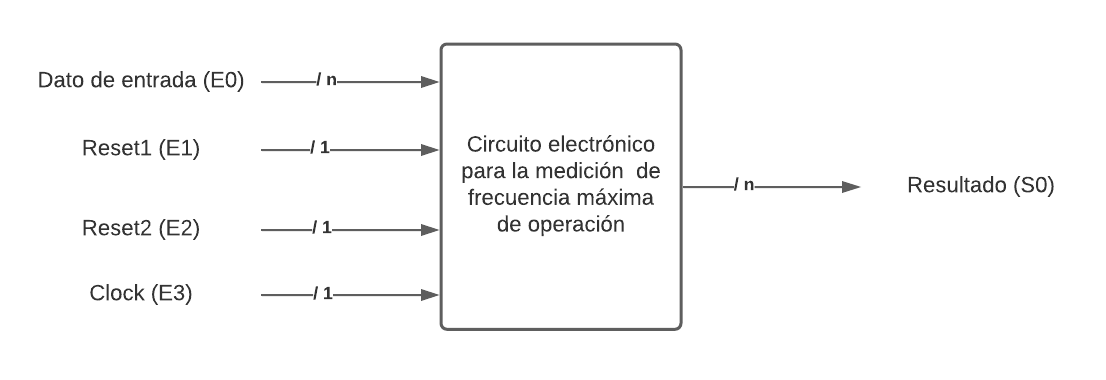
\includegraphics[scale = 0.4]{img/nivel12.png}
		\caption{Diagrama de primer nivel del circuito electrónico para la medición  de frecuencia máxima de operación}
		\label{fig:niv12}
	\end{figure}
	
	
	En la Figura \ref{fig:niv22}, se puede observar el diagrama de segundo nivel del circuito electrónico para la medición de frecuencia máxima de operación; dicho diagrama consta de 3 submódulos principales: el primero de ellos es el Registro 1, este consta de la entrada E0 (Dato de entrada) es de n bits, la entrada E1 (Reset1) es el reset para el primer registro es de 1 bit y la entrada E3 (Clock) es una entrada en común de reloj para ambos registros y es de 1 bit; así mismo tiene la salida de este módulo que es OutR1 y esta es ambos números introducidos y guardados en el Registro 1. Al ALU le entra esa salida del Registro 1 (OutR1) con los dos números a operar y genera una salida OutALU con el resultado de la operación. Y finalmente el Registro 2 posee la entrada E2 (Reset2) es el reset para el segundo registro es de 1 bit, la entrada E3 (Clock) es una entrada en común de reloj para ambos registros y es de 1 bit y la entrada OutALU, proveniente de la salida del ALU; su salida correspondiente es Resultado (S0) y es de n bits. Como se ha estudiado e investigado anteriormente, la función de los registros es almacenar un valor, cuando se activa una señal.
	
	Por otro lado, el mismo circuito sólo posee una salida la cual es el Resultado (S0) y es de n bits, este hace referencia al resultado de operar los dos números en el ALU.  la entrada E2 (Reset2) es el reset para el segundo registro es de 1 bit
	
	\begin{figure}[hbtp]
		\centering
		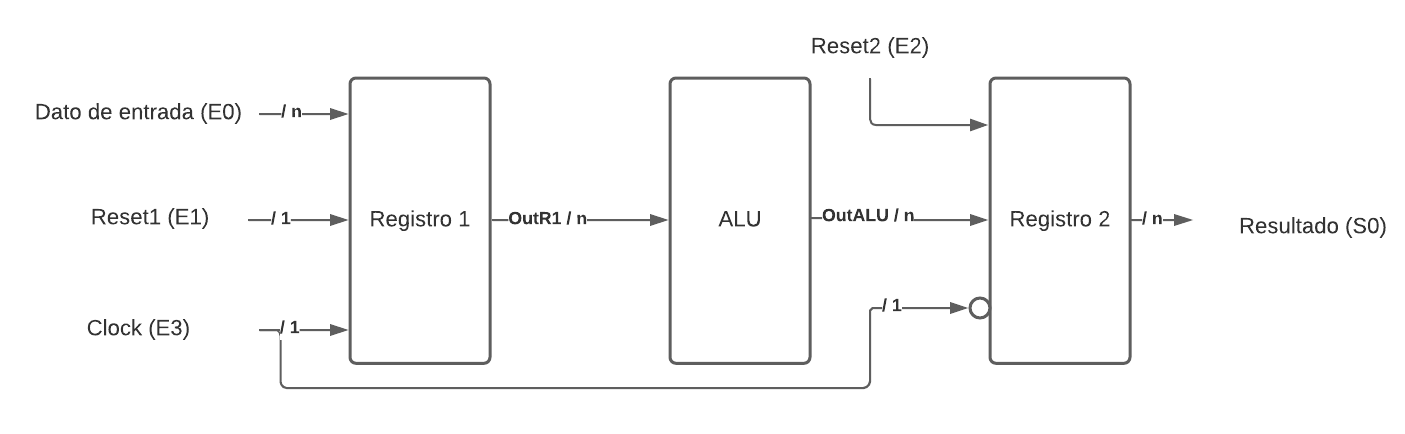
\includegraphics[scale = 0.37]{img/nivel22.png}
		\caption{Diagrama de segundo nivel del circuito electrónico para la medición  de frecuencia máxima de operación}
		\label{fig:niv22}
	\end{figure}
	
	\section{Resultados}
	
	\subsection{Experimento 1}
	
	Al realizar el experimento 1 de este laboratorio, se realizaron testbench de autochequeo para cada uno de los módulos implementados en la ALU.
	En la Figura \ref{fig:wsum}, se puede observar la salida de onda del tesbench para el módulo del sumador implementado en la ALU.
	
	\begin{figure}[hbtp]
		\centering
		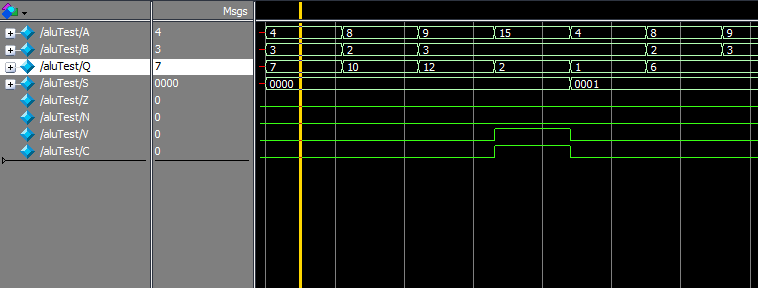
\includegraphics[scale = 0.4]{img/wsumador.png}
		\caption{Onda de salida del sumador en la ALU}
		\label{fig:wsum}
	\end{figure}
	
	En la Figura \ref{fig:wres}, se puede observar la salida de onda del tesbench para el módulo del restador implementado en la ALU.
	
	\begin{figure}[hbtp]
		\centering
		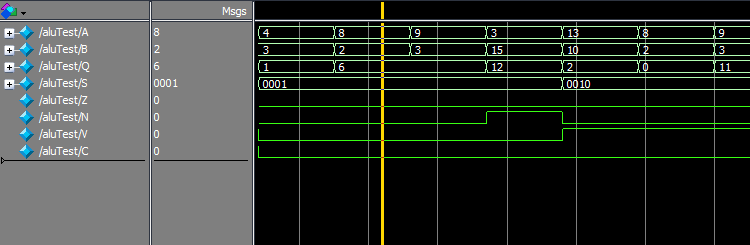
\includegraphics[scale = 0.4]{img/wrestador.png}
		\caption{Onda de salida del restador en la ALU}
		\label{fig:wres}
	\end{figure}
	
	En la Figura \ref{fig:wmul}, se puede observar la salida de onda del tesbench para el módulo de la multiplicación implementado en la ALU.
	
	\begin{figure}[hbtp]
		\centering
		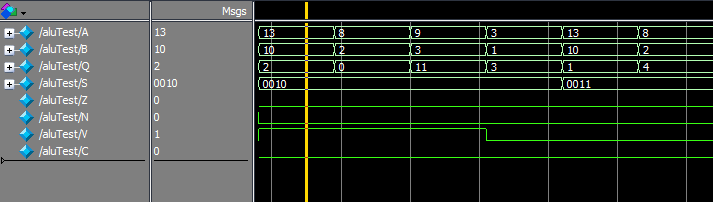
\includegraphics[scale = 0.4]{img/wmultiplicacion.png}
		\caption{Onda de salida de la multiplicación en la ALU}
		\label{fig:wmul}
	\end{figure}
	
	En la Figura \ref{fig:wdiv}, se puede observar la salida de onda del tesbench para el módulo de la división implementado en la ALU.
	
	\begin{figure}[hbtp]
		\centering
		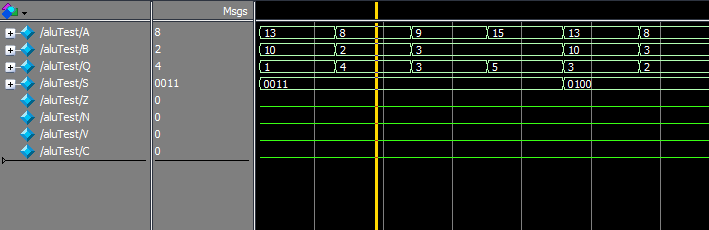
\includegraphics[scale = 0.4]{img/wdivision.png}
		\caption{Onda de salida de la división en la ALU}
		\label{fig:wdiv}
	\end{figure}
	
	En la Figura \ref{fig:wmod}, se puede observar la salida de onda del tesbench para el módulo del módulo o residuo implementado en la ALU.
	
	\begin{figure}[hbtp]
		\centering
		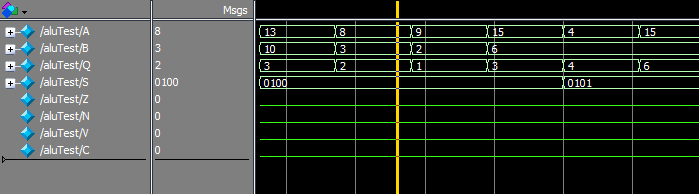
\includegraphics[scale = 0.4]{img/wmodulo.png}
		\caption{Onda de salida del residuo o módulo en la ALU}
		\label{fig:wmod}
	\end{figure}
	
	En la Figura \ref{fig:wand}, se puede observar la salida de onda del tesbench para el módulo de la compuerta AND implementado en la ALU.
	
	\begin{figure}[hbtp]
		\centering
		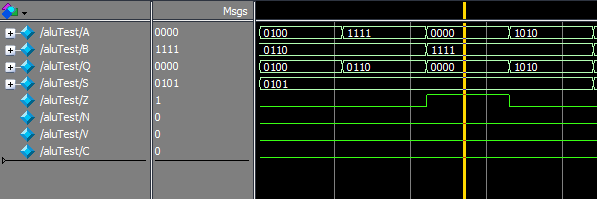
\includegraphics[scale = 0.5]{img/wand.png}
		\caption{Onda de salida de la compuerta AND en la ALU}
		\label{fig:wand}
	\end{figure}
	
	En la Figura \ref{fig:wor}, se puede observar la salida de onda del tesbench para el módulo de la compuerta OR implementado en la ALU.
	
	\begin{figure}[hbtp]
		\centering
		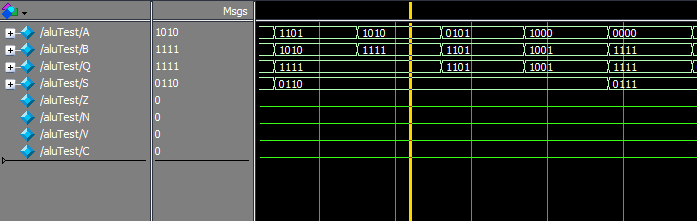
\includegraphics[scale = 0.4]{img/wor.png}
		\caption{Onda de salida de la compuerta OR en la ALU}
		\label{fig:wor}
	\end{figure}
	
	En la Figura \ref{fig:wxor}, se puede observar la salida de onda del tesbench para el módulo de la compuerta XOR implementado en la ALU.
	
	\begin{figure}[hbtp]
		\centering
		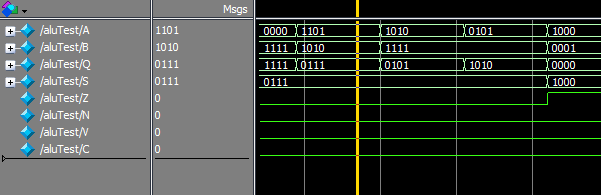
\includegraphics[scale = 0.5]{img/wxor.png}
		\caption{Onda de salida de la compuerta XOR en la ALU}
		\label{fig:wxor}
	\end{figure}
	
	En la Figura \ref{fig:wsl}, se puede observar la salida de onda del tesbench para el módulo del shift left implementado en la ALU.
	
	\begin{figure}[hbtp]
		\centering
		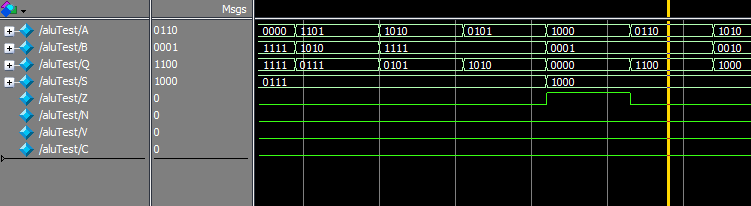
\includegraphics[scale = 0.4]{img/wsl.png}
		\caption{Onda de salida del shift left en la ALU}
		\label{fig:wsl}
	\end{figure}
	
	En la Figura \ref{fig:wsr}, se puede observar la salida de onda del tesbench para el módulo del shift right implementado en la ALU.
	
	\begin{figure}[hbtp]
		\centering
		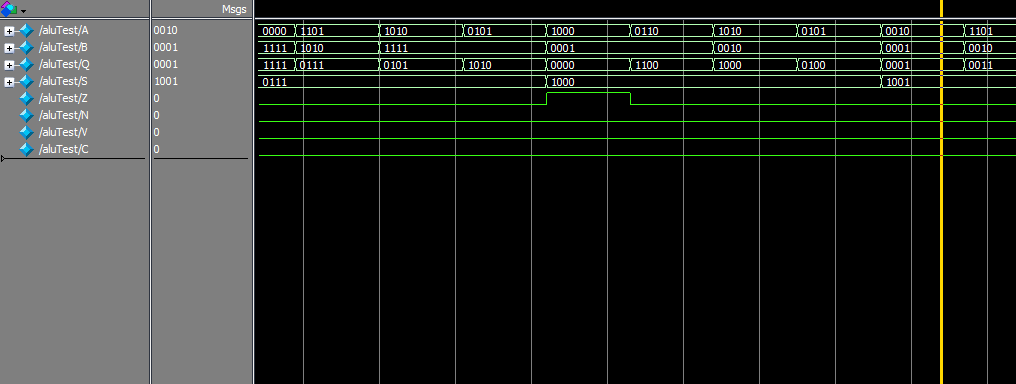
\includegraphics[scale = 0.3]{img/wsr.png}
		\caption{Onda de salida del shift right en la ALU}
		\label{fig:wsr}
	\end{figure}
	
	En la Figura \ref{fig:niv31}, se puede observar el diagrama generado por Quartus de la unidad aritmética lógica (ALU).
	
	\begin{figure}[hbtp]
		\centering
		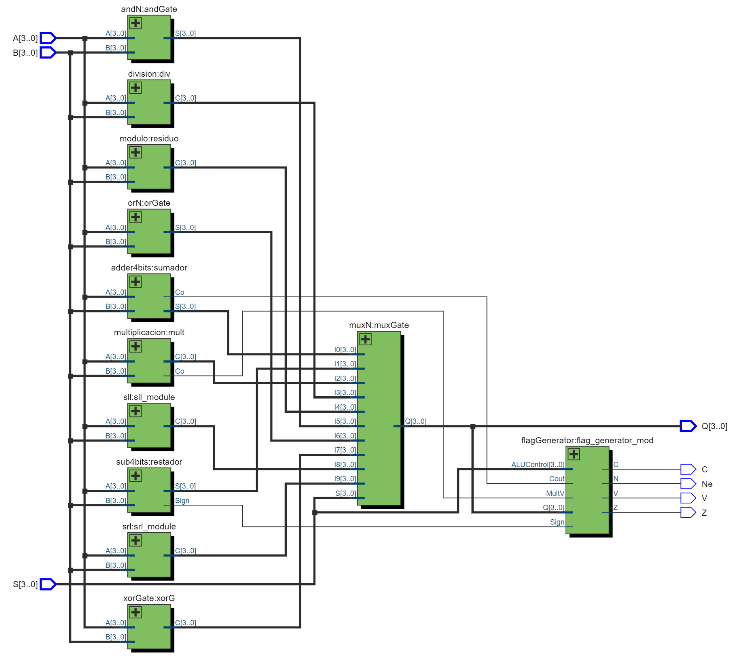
\includegraphics[scale = 0.45]{img/nivel31.PNG}
		\caption{Diagrama generado por Quartus del ALU}
		\label{fig:niv31}
	\end{figure}
	
	
	\subsection{Experimento 2}
	
	Al realizar este experimento, se obtuvieron los datos que se encuentra en la Tabla VI, en la cual se puede apreciar la cantidad de ALMs, la cantidad de registros utilizados, la cantidad de bits de entrada y la frecuencia máxima. 
	
	\begin{table}[hbtp]
		\begin{center}
			\caption{Tabla de las operaciones con su respectivo selector.}
			\label{tab:tablaf}
			
			\begin{tabular}{c | c | c | c | c }
				\hline
				\textbf{Bits de entrada} & \textbf{ALMs} & \textbf{Registros} &
				\textbf{Pines} &
				\textbf{Frecuencia (max)} \\
				\hline 10 & 4 & 15 & 22 & 380.23 MHz  \\
				\hline  32 & 13 & 48 & 66 & 369.28 MHz  \\
				\hline 64 & 25 & 96 & 130 & 375.94 MHz \\
				\hline 128 & 49 & 192 & 258 & 374.53 MHz\\
				\hline 256 & 193 & 384 & 514 & ---  \\
			\end{tabular}
		\end{center}
	\end{table}
	
	\begin{figure}[hbtp]
		\centering
		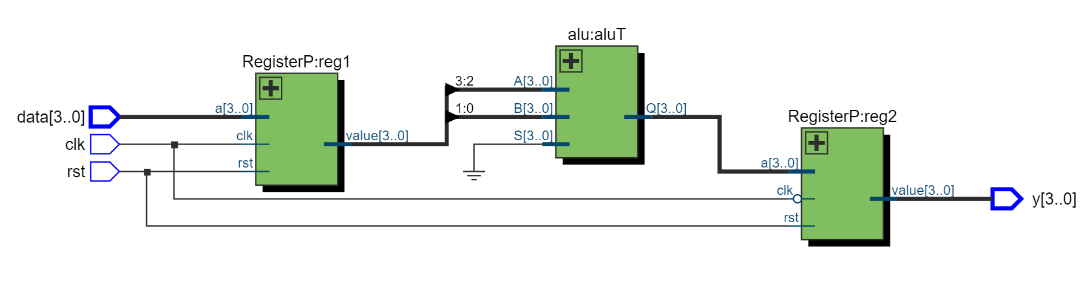
\includegraphics[scale = 0.3]{img/nivel32.PNG}
		\caption{Diagrama generado por Quartus del ALU, al utilizar dos registros}
		\label{fig:niv32}
	\end{figure}
	
	\begin{figure}[hbtp]
		\centering
		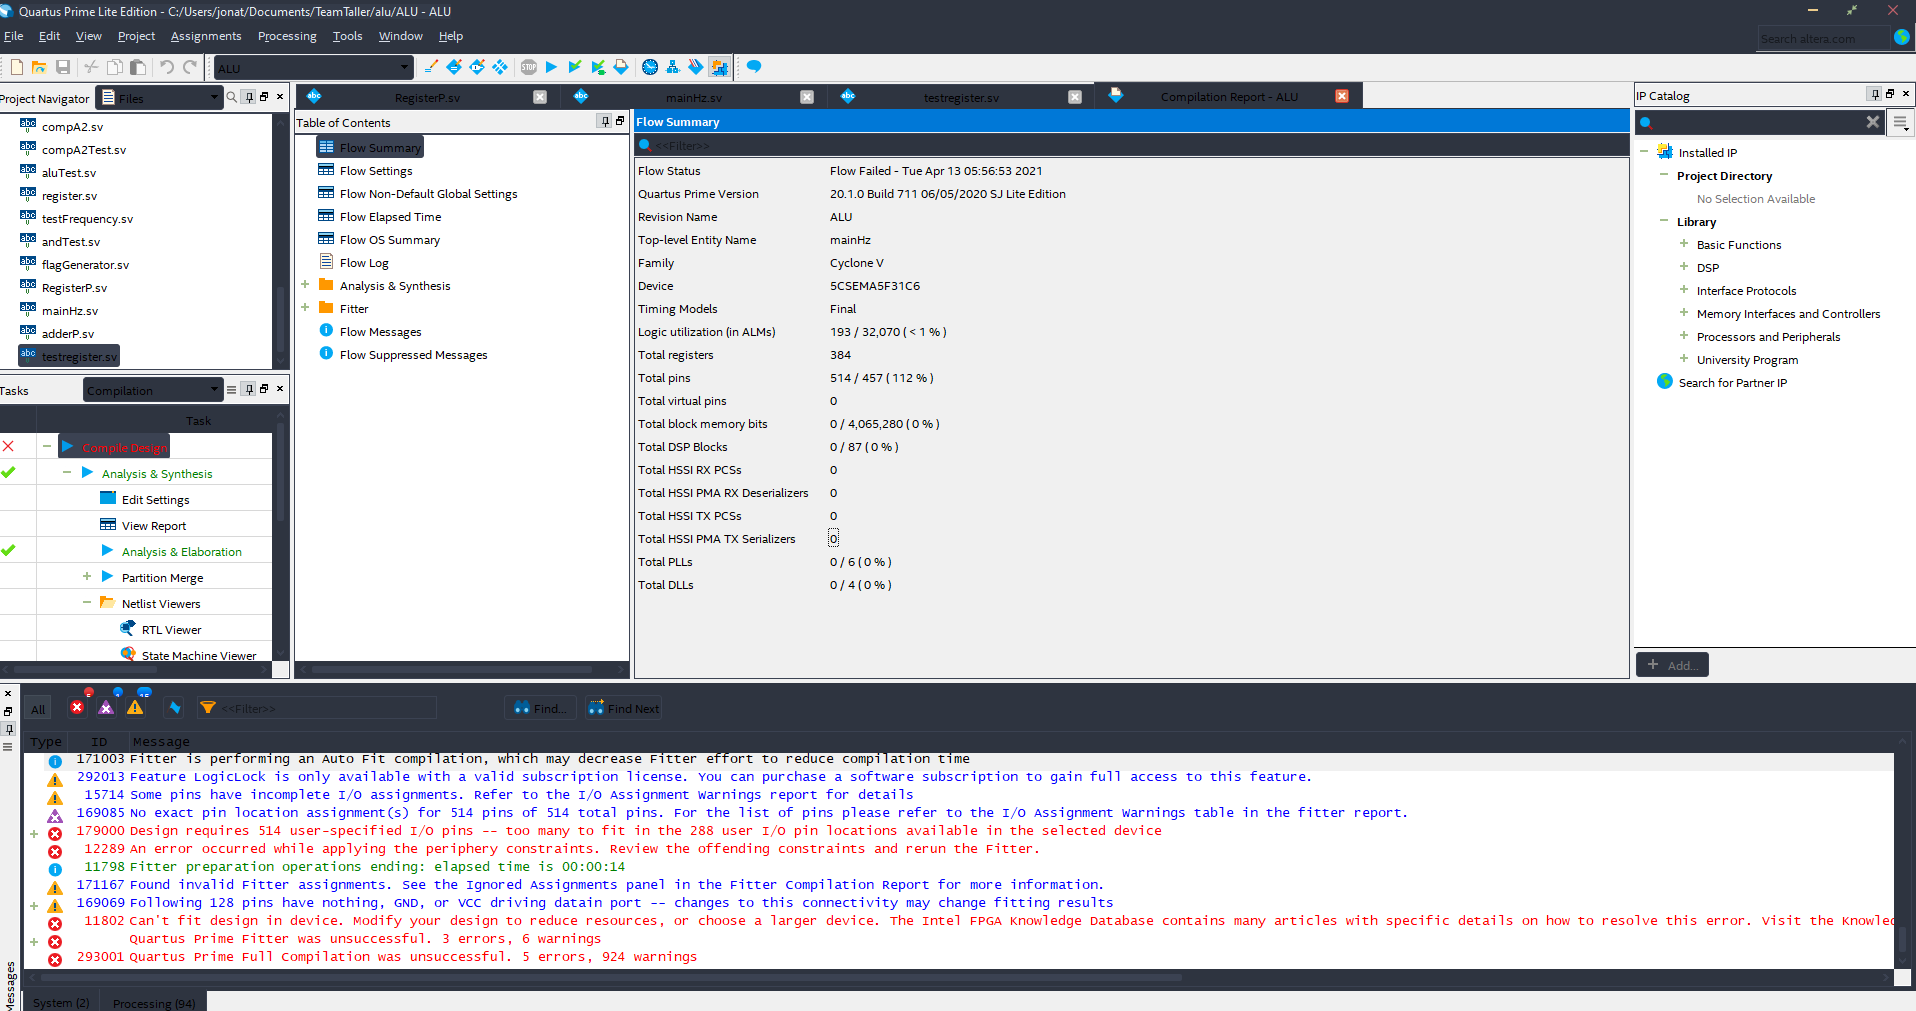
\includegraphics[scale = 0.12]{img/error.png}
		\caption{Error generado al tratar de introducir 256 bits en el ALU, para implementarlo en la FPGA}
		\label{fig:err}
	\end{figure}
	
	\section{Análisis de resultados} 
	
	\subsection {Experimento 1}
	Tal como se puede observar en la Figura \ref{fig:wsum} como al sumar los números binarios: $0100$ y $0011$, su salida es operada correctamente por el módulo sumador que se encuentra en la ALU y su resultado es de $0111$.
	
	En la Figura \ref{fig:wres} como al restar los números binarios: $0011$ y $1111$, su salida es operada correctamente por el módulo restador que se encuentra en la ALU y su resultado es de $1100$, además pone en alto la bandera del Negativo. 
	
	En la Figura \ref{fig:wmul} como al multiplicar los números binarios: $1001$ y $0011$, su salida es operada correctamente por el módulo de multiplicación que se encuentra en la ALU y su resultado es de $1011$, además pone en alto la bandera de Overflow.
	
	En la Figura \ref{fig:wdiv} como al sacar la división entera de los números binarios: $1101$ y $1010$, su salida es operada correctamente por el módulo división que se encuentra en la ALU y su resultado es de $0001$.
	
	En la Figura \ref{fig:wmod} como al sacar el residuo de los números binarios: $1101$ y $1010$, su salida es operada correctamente por el módulo modulo que se encuentra en la ALU y su resultado es de $0011$.
	
	En la Figura \ref{fig:wdiv} como al sacar la operación lógica AND de los números binarios: $0101$ y $0100$, su salida es operada correctamente por el módulo andN que se encuentra en la ALU y su resultado es de $0100$.
	
	En la Figura \ref{fig:wdiv} como al sacar la operación lógica OR de los números binarios: $1101$ y $1010$, su salida es operada correctamente por el módulo orN que se encuentra en la ALU y su resultado es de $1111$.
	
	En la Figura \ref{fig:wdiv} como al sacar la operación lógica XOR de los números binarios: $1101$ y $1010$, su salida es operada correctamente por el módulo xorN que se encuentra en la ALU y su resultado es de $0111$.
	
	En la Figura \ref{fig:wsl} como al sacar el shift left de los números binarios: $1000$ y $0001$, su salida es operada correctamente por el módulo shiftLeft que se encuentra en la ALU y su resultado es de $0000$.
	
	En la Figura \ref{fig:wsr} como al sacar el shift right de los números binarios: $1101$ y $0010$, su salida es operada correctamente por el módulo shiftRight que se encuentra en la ALU y su resultado es de $0011$.
	
	Con cada una de estas pruebas generadas en el testbench de auto chequeo de la unidad aritmética lógica, se puede comprobar el adecuado funcionamiento de cada uno de los módulos de la misma.
	
	Como se puede observar en la Figura \ref{fig:niv31}, el diagrama generado por Quartus corresponde y es equivalente al diagrama que fue generado en la sección de Desarrollo en donde sale cada uno de los módulos que contiene la ALU, con su respectiva entrada de selección, el MUX y el generador de banderas.
	
	\subsection{Experimento 2}
	
	Como se puede observar en la Tabla VI, al aumentar la cantidad de bits en la entrada del ALU, aumenta la cantidad de ALMs, la cantidad de Registros y de Pines que se utilizan en la FPGA; con esto se puede probar cómo al aumentar la cantidad de bits en la entrada, la FPGA consume más recursos. 
	
	Al querer implementar la ALU con 256 bits de entrada, se consumen todos los recursos de la FPGA y no existen pines suficientes, ya que la misma indica que se está consumiendo un 112 porciento, por lo cual es imposible utilizar 256 bits de entrada.
	
	Con los resultados y datos obtenidos en la Tabla VI, se puede observar como la máxima frecuencia en la cual puede operar es de $389.23 MHZ$, la cual hace referencia a los 10 bits de entrada, esto se debe a que la frecuencia es inversamente proporcional al tiempo y con 10 bits, la ejecución de las operaciones es menor que con una mayor cantidad de bits.
	
	Como se puede observar en la Figura \ref{fig:niv32}, el diagrama generado por Quartus corresponde y es equivalente al diagrama que fue generado en la sección de Desarrollo (Figura \ref{fig:niv22}) en donde sale cada uno de los dos registros así como el ALU, con sus respectivas entradas de reset, y clock.
	
	En la Figura \ref{fig:err}, se puede observar como al tratar de introducir 256 bit, Quartus genera un error, porque no hay pines suficientes para poder implementar dicho programa.
	
	\begin{figure}[hbtp]
		\centering
		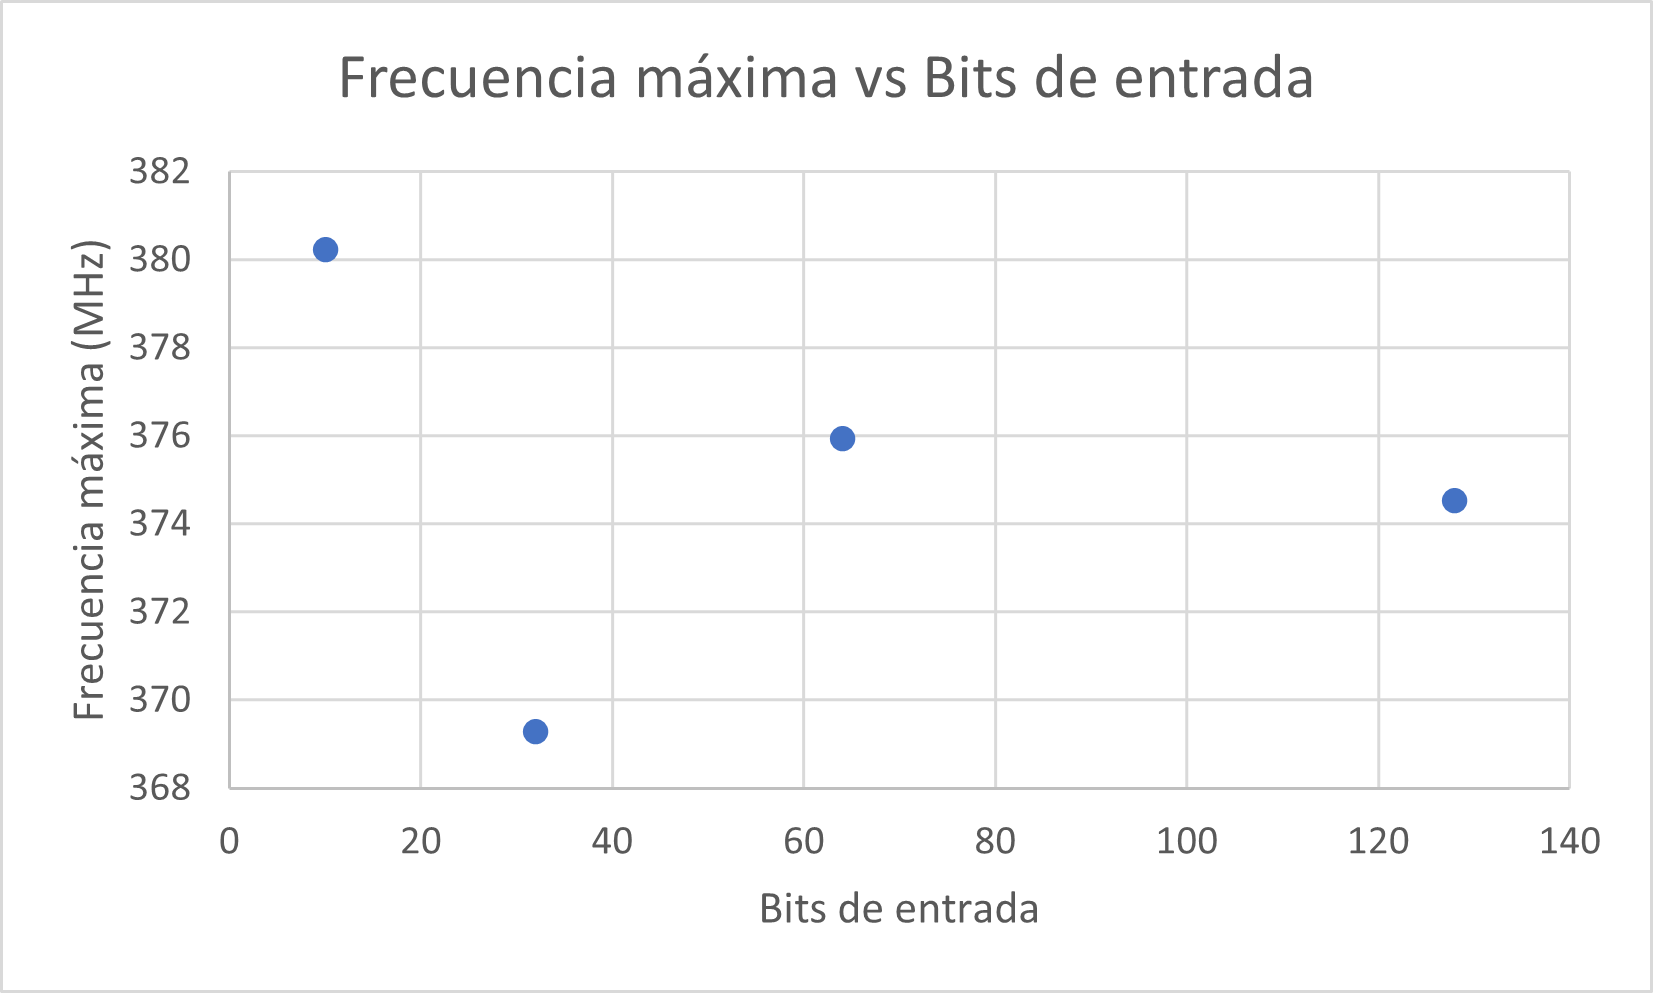
\includegraphics[scale = 0.65]{img/chart1.png}
		\caption{Gráfico de frecuencia máxima vs bits de entrada}
		\label{fig:cha}
	\end{figure}
	
	En la Figura \ref{fig:cha}, se observa la tendencia que tienen los puntos del gráfico a decrecer, esto se presenta porque la frecuencia delimita al tiempo de propagación y cada vez que se aumentan los bits de entrada, se consumen más recursos de la FPGA como ALMs, registros y pines, lo que provoca que el tiempo de respuesta sea más lento  y más larga la ruta crítica que pueden tomar los datos.
	
	\section{Conclusiones}
	
	\section{Bibliografía}
	
	\bibliographystyle{IEEEtran}
	\bibliography{myref}
	
\end{document}